
% We have demonstrated that tuning a pipline specifically for a BNS search has yieled  
% a significant improvment in sensitivity as compared to naive tunings based on a larger
% parameter space. While these are sensitive to the specific noise characteristics 
% of the detector, which will be different (broader and lower) in Advanced LIGO
% we can extrapolate that these same tuning choices will be important to revisit in the 
% first weeks of analysis. 

% I suggest also testing with sensitivites with the recolored data as well on the final
% tuning choice

\section{Introduction}
\label{sec:introduction}

We present an offline search pipeline tuned for the detection of gravitational-waves from binary neutron start sources, and show that this targeted search yields significant improvements in sensitivity to BNS sources. Whereas in prior searches for BNS systems, such as the last one conducted in S6/VSR2,3, a non-spinning template bank was constructed that contained masses up to $25M_\odot$ ~\cite{Abadie:2011nz} and was tuned to maxize the overall sensitivity, in this work we focus solely on BNS systems with a mass range from $1-3 M_\odot$. We consider two banks of templates, a \emph{non-spinning template bank} designed to be sensitive to mergers where the components have neglible intrinsic angular moment, and an \emph{aligned spin template bank} which is designed to be sensitive to BNS mergers where the intrinsic angular momentum of the components can be as large as $\chi=0.4$. To approximate the conditions of the first observing run with Advanced LIGO, we focus on a two-detector network composed of the Hanford (LHO) and Livingston (LLO) observatories. To assess proposed improvements to the search pipeline we test the search on three weeks of LIGO data from S6.

This chapter is organized as follows. In sec.~\ref{sec:pipeline} we describe the methodology of the search pipeline, and we present a method for estimating the significance of candidate events. In sec.~\ref{sec:tuning}, starting with the configuration suggested in chapter~\ref{ch:single_stage}, which improved upon the S6/VSR2,3 by requiring exact-match coincidence, we present a procedure for further improving the search sensitivity of the pipeline by optimizing key parameters of the search, namely the configuration of the power spectral estimation, the signal-consistency tests, the single detector SNR thresholds, and the lower frequency cutoff. 

\section{Significance of Candidate Events}
\label{sec:pipeline}

The focused BNS search pipeline implements the single stage analysis pipeline proposed in chapter~\ref{ch:single_stage}. A bank of post-Newtonian TaylorF2 3.5 PN order templates, generated using the metric based placement algorithm proposed in chapter~\ref{ch:bns_spin}, is created to span the extended binary neutron star mass range from $1-3 M_\odot$. A template bank is generated separately for each of the three S6/VSR2,3 analysis weeks, using the harmonic mean of the detector data during that week. Each template is match-filtered against the data to calculate a signal-to-noise time series. Excursions in the SNR time series from each detector are recorded if they exceed a fixed SNR threshold, which was 5.5 in S6/VSR2,3, and it is the loudest within one second. To cope with the large number of transient non-Gaussian events, we apply a signal consistency test, and calculate a reweighted signal-to-noise ratio, defined in \ref{eq:newSNR}.

We additionally require that a candidate is seen by both the Hanford and Livingston observatories. In keeping with the findings of Ch.~\ref{ch:single_stage} we require that the trigger in each detector be found by the same template, and within the light-travel time between the detectors. A combination of single detector events that passes this test is a \emph{coincident event}, whose combined statistic is given by Eq.~\ref{eq:cnewsnr}.

In order to claim a candidate signal as the detection of a gravitational-wave, we need to determine the probability that it could have been due to noise. We estimate the false alarm rate by forming coincidences between single detector triggers that are outside of the standard coincident time window. For both computational efficiency and simplicity, we choose to form background coincidences by applying a time shift to one detector. The triggers from one detector are offset by all possible non-zero integer multiples of a fixed interval, $T_s$, known as the \emph{timeslide interval}. For this analysis, we haven chosen $T_s$ to be 0.2 s. From these time slides, we collect a set of coincident triggers. As this set was formed from all of the original single detector triggers, we will refer to it as the \textit{inclusive background}, $B_{inc}$. Note, that if there is a loud gravitational-wave signal its component single detector triggers will also form coincidences with noise triggers from the other detector, and those will be contained in this background set. The inclusive set of background triggers can be expanded as
%
\begin{equation}
B_{inc} = \{N_H \oplus N_L\} \cup \{ N_H \oplus S_L \} \cup \{S_H \oplus N_L\},
\end{equation}
where $N_{H/L}$ are single detector noise triggers, $S_{H/L}$ are single detector triggers from gravitational-wave signals, and $\{A \oplus B\}$ represents the set of coincidences between the single detector triggers A and B. We can define a set of background triggers that excludes coincidences between signals and noise, $B_{exc}$, by excising single detector time surrounding each of the foreground coincident triggers, with components $F_H$ and $F_L$. We refer to the amount of time ingored as the \emph{blinding window}, $T_{blind}$, which in this case we have chosen to be 100ms. This can be expressed as,
%
\begin{equation}
B_{exc} = B_{inc} - \{S_H \oplus T_L\} - \{R_H \oplus S_L\} - \{S_H \oplus R_L\},
\end{equation}
%
where $R_{L/H} \in N_{L/H}$, and the time difference between any element in $R_{L/H}$ and any element of $F_{H/L}$ is greater than the blinding window $T_{blind}$. This is chosen as a balance between the amount of triggers removed and the influence that a gravitational-wave signal may have on the template. 

Both backgrounds are valid for different types of questions. The inclusive background admits the possibility that all triggers could be noise generated, including the triggers of a candidate signal. The exclusive background presumes that a given candidate is a signal while testing it against the remainder of the background. Estimating the significance of a candidate by comparing against the inclusive background will result in a more conservative value. During the S6/VSR2,3 search, ~\cite{Collaboration:2011np}.

We use the false alarm rate as our principle measure of the significance of a candidate event. Given an event wih a $\rho^c_{new}=x$, we can express the false alarm rate (FAR), when comparing to both the inclusive and exclusive background sets as
%
\begin{equation}
FAR (x) = N (x) / {T_B},
\end{equation}
%
where $N(x)$ is the number of coincident events in the estimated background set with a $\rho^c_{new} > x$. A separate FAR is calculated using both the inclusive and exclusive background sets, giving two significance measures, $FAR_{inc}$ and $FAR_{exc}$. $T_B$ is the effective background time, which can be accurately estimated from the single-detector livetimes $T_H$ and $T_L$ for the Hanford and Livingston detectors, respectively, as
%
\begin{eqnarray}
T_B =  T_H \times T_H / T_s
\end{eqnarray}
%
Note, that this is not an exact calculation of the background livetime. The exact time can be obtained by explicitly calculating the amount of overlapping time between the Hanford and Livingston gravitational-wave data for each time slide and taking the sum. The estimate is equivelant to the exact calculation in the case that the start and end of every chunck of analyzed data lies on multiple of the timeslide interval. As such, we can calculate the upper bound on the difference between the true and estimated value of the background livetime as
%
\begin{eqnarray}
|T_{b, estimate} - T_{b, exact} |< 2 \times N_{chunks} \times T_s,
\end{eqnarray}
%
where $N_{chunks}$ is the number of non-contigious analysis chunks. As our analysis discards chunks of data that are less than 2048 seconds in length, and  $T_s=200$ ms, the relative error is strictly less than $.02\%$, and so can safely be considered negligible.

\section{Optimizing Search Sensitivity}
\label{sec:tuning}

In this section, we retune several parameters of the CBC search, with the aim of creating a search optimized for the detection of binary neutron star mergers. The potential parameter space of tuning choices is quite large, so we have started with the filtering settings used in the lowmass CBC search performed in S6/VSR23, and include the proposed changes from Ch. \ref{ch:single_stage}. 

In the following sections, we test proposed changes to the analysis pipeline using a template bank which is designed to have a $97\%$ minimal match with non-spinning BNS signals with component masses between $1-3 \M_\odot$. We evalutate the search performance of a particular set of tuning parameters, by using the  sensitive volume of the search integrated over the coincident livetime of each of our three sample weeks of S6 data. The sensitive volume is estimated by simulating a population of sources, inserting them into real detector data, and recovering them using the search pipeline. In this work, we choose the test injection set to consist of non-spinning BNS sources distributed uniformly between $1-3 \M_\odot$.

The product of the sensitive volume and the coincident ananlysis time, $VT$, can be expressed as,
%
\begin{eqnarray}
VT (F) = \sum_{w=0}^2 V(w, F) T_{coinc}(w)
\end{eqnarray}
%
where V(w, F) is the sensitive volume as given by Eq.~\ref{eq:sensitive_volume} for a given week, $w$, of the sample analysis. The total amount of analysis time for a given week is given by $T_{coinc}(w)$. The quanitity VT is directly proportional to the expected number of detected gravitaional-wave signals from the simulated population. 

\subsection{Power Spectrum Estimation}
\label{sec:psd}

Because the overall sensitivity of a detector, along with the shape of its power spectral density (PSD) changes over time, the spectral density used to calculated the matched-filtering SNR of candidate events is periodically recalculated. The S6/VSR2,3 analysis recomputed the PSD using every 1920 seconds, an interval known as the \emph{analysis chunk}. However, due to the additional padding required for filtering, 2048s of data was used for each PSD estimate. Every 2048s chunk of data was subdivided into 15 segments, each with 256s duration and overlapped by 50$\%$. The PSD of each analysis chunk is calculated by first taking the median average of the Fourier transform of each segment. Finally, we truncate the inverse of the PSD in the time domain to restrict the filter corruption to a fixed length of time. In addition, this has the effect of smoothing out lines within the spectrum. An inverse truncation value of 16 seconds was used throughout S6/VSR2,3. 

We investigate a straightforward improvement to this algorithm. Instead of calculating the PSD using 256 second segments and applying a 16 second inverse spectrum truncation, we propose calculating the PSD using 16 second segments directly, interpolating for the intended use case, and finally applying the same 16s inverse spectrum truncation. Increasing the number of samples in the PSD estimate decreases the variance, and reduces the influence of outliers. The results of this investigation are shown in figure Fig.~\ref{fig:psd}, where the sensitive volume-time is compared for the initial reference configuration and for the proposed configuration as a function of the inverse false alarm rate. The proposed PSD estimation shows clear improvement over the method used in S6/VSR2,3, resulting in an average $\approx 12\%$ increase in sensitivity between inverse false alarm rates of $10^3$ and $10^4$ years.  

%In this section, we investigate a straightforward improvement to the estimation of PSDs %within the search pipeline.

%This value is chosen to be as small as possible to limit the amount of data removed due to filter startup time, but large enough so that the PSD estimate itself can capture the complex behavior of the numerous frequency lines. For S6 data this was chosen to be 16 seconds. Due to technical limitations, not scientific ones, the length of the PSD estimate was chosen to be 256 seconds. 

%Using a newer pipeline that has removed these limitations, we investigate the benefit of directly measure the PSD in 16 second intervals, given that this satisfies the same constraint on correlation length. The allows an increased number of PSD estimates from 15 to ~250, which has a impact on the variance of the PSD estimate. (how much??). 

\begin{figure}
\centering
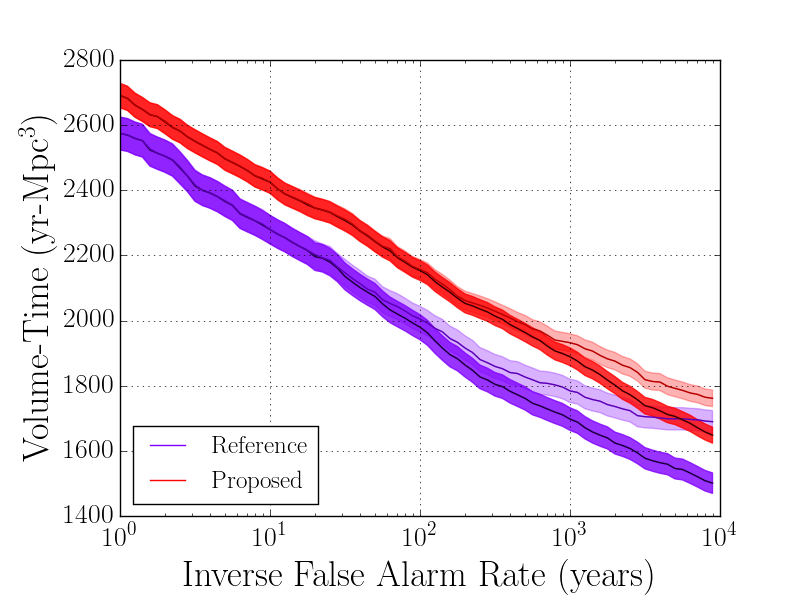
\includegraphics[width=1.0\textwidth]{papers/bns_o1_dev/figures/psd_combined.png}
\caption{\label{fig:psd} 
The combined VT as a function of inverse false alarm rate, for the combined three weeks of analysis, and for an injection population that uniformly covers the parameter space of the non-spinning BNS region, with component masses between $1- 3M_\odot$. Darker colored lines indicate the inclusive IFAR value, while lighter lines show the exclusive IFAR. The reference (red) PSD estimation uses 15, 256s segments. The proposed (purple) tuning which uses 252, 16s segments. Both truncate the inverse spectrum in the time domain to 16 seconds. The proposed configuration improves the search sensitivity by $\approx 12\% $ at a false alarm rate of 1 per 1000 years.
}
\end{figure}

\subsection{Signal-to-noise Threshold}
\label{sec:snr}

For each detector, triggers are recorded when the signal-to-noise ratio exceeds a pre-determined threshold, $\rho_t$. For the S6/VSR2,3 CBC search, only triggers with an SNR above 5.5 were recorded. Beginning with the PSD tunings proposed in sec.~\ref{sec:psd}, we investigate the effect of lowering the SNR threshold to 5.0. A comparison of the search sensitivity at $\rho_t=5.5$ and $\rho_t=5.0$ is shown in Fig.~\ref{fig:snrthreshold}. We see that lowering $\rho_t$ from 5.5 to 5.0 has not resulted in a significant improvement in sensitivity. We observe that at high inverse false alarm rate, the inclusive IFAR is identical between the two thresholds, but that there is a very minor increase in sensitivity when using the exclusive IFAR.

In Fig.~\ref{fig:ifarifar} we explore where the differences between the inclusive and exclusive IFAR estimates are the greatest. At a fixed exclusive IFAR, which monotonically increases with the combined weighted SNR of an injection trigger, we find that there is an inverse relation between the inclusive IFAR and the minimum single detector SNR. This indicates that lowering the SNR threshold below $\approx 5.3$ will not yield an improvement in sensitivity at inclusieve false alarm rate of 1 in 1000 years, for a two-detector search composed of the Hanford and Livingston LIGO observatories. Note that this result cannot be generalized to a multi-detector network, where there can be a non-trivial increase in detection confidence due to the presence of quiet trigger in the additional detectors. Further work is required to characterize the appropriate SNR thresholds for multi-detector networks.

%maybe add ranking stat to the right axis of this plot?


\begin{figure}
\centering
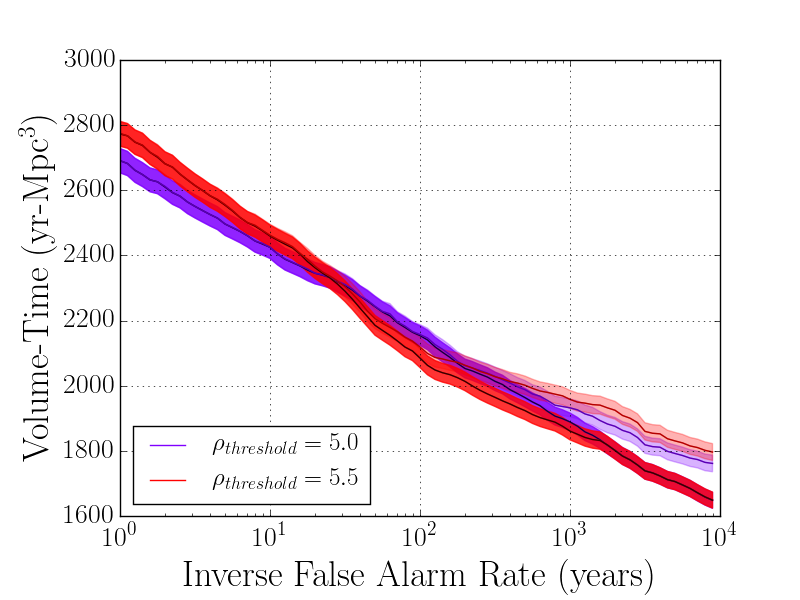
\includegraphics[width=1.0\textwidth]{papers/bns_o1_dev/figures/snr_combined.png}
\caption{\label{fig:snrthreshold} 
The combined VT as a function of inverse false alarm rate, for the combined three weeks of analysis, and for an injection population that uniformly covers the parameter space of the non-spinning BNS region, with component masses between $1- 3M_\odot$. Darker shaded lines indicate the inclusive IFAR value, while lighter lines show the exclusive IFAR. We find that dropping the SNR threshold of the analysis from 5.5 (red) to 5.0 (purple) has a negligible effect on the overall search sensitivity.
}
\end{figure}

\begin{figure}
\centering
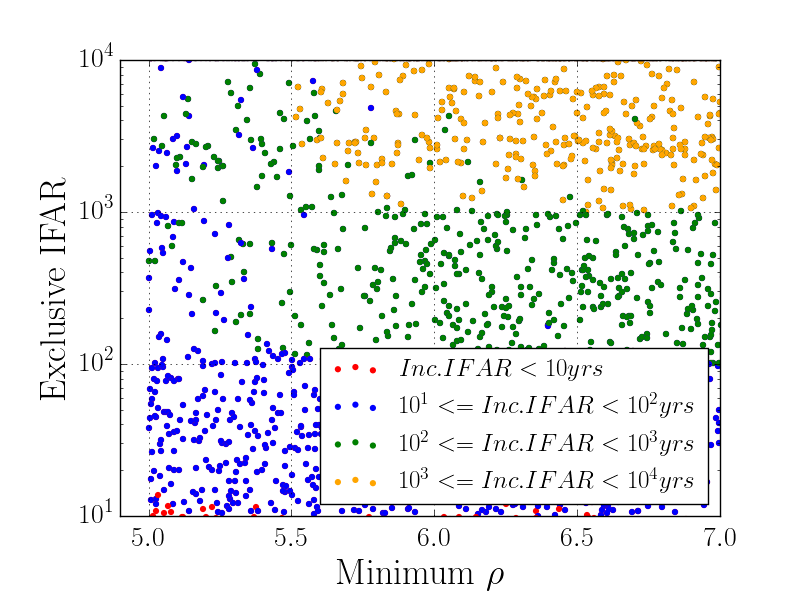
\includegraphics[width=1.0\textwidth]{papers/bns_o1_dev/figures/ifarifar.png}
\caption{\label{fig:ifarifar} 
The distribution of exclusive IFAR as a function of the minumum single detector SNR, for an injection population that uniformly covers the parameter space of the non-spinning BNS region, with component masses between $1- 3M_\odot$. Injections are colored by the value of their inclusive IFAR. We observe that there is an inverse relationship between the inclusive IFAR and the minimum SNR value. This indicates that for a given value of inclusive IFAR, there is a corresponding SNR threshold, below which, the search sensitivity as function of inclusive IFAR will not improve
}
\end{figure}


\subsection{Signal-consistency Test and Ranking Statistic}
\label{sec:chisq}

As detailed in Ch.~\ref{ch:search}, the single-detector ranking statistic is the SNR weighted by a time-frequency signal consistency test. The test breaks a template into $p$  frequency bins of each power. Although the boundaries of the bins are defined in the frequency domain, as the TaylorF2 templates we use in the analysis are a monotonic functions of time and frequency, we can outline the rough time-frequency boundaries of each bin as demonstrated in Fig.~\ref{fig:chisqbins}. We show the 16 bins used in the S6/VSR2,3 analysis. Since the response of the time-frequency chisq is dependent on the morphology of the non-Guassian noise present in the data, we investigate if increasing the number of time-frequency bins for a BNS focused search, where the average template duration is significantly longer than for searches that include higher mass templates, has an effect on the search sensitivity.

Starting with the analysis tunings suggested in \ref{sec:snr}, we compare the search sensitivity at a fixed exclusive FAR of 1 per 1000 years. The results in Fig.~\ref{fig:vbin}, show that increasing the number of time-frequency bins from 16 to 64-256 results in an $\approx 12\%$ improvement in search sensitivity. From the results of Fig~.\ref{fig:fchisq} we see  that this improvement occurs at all values of the FAR. Based on this result, we propose using a value of 128 bins for a BNS analysis, but would suggest re-examining this choice as the effective length of a BNS template increases as detectors such as Advanced LIGO proceed towards design sensitivity.

%The primary ranking statistic we use is "NewSNR". It is a chisq-weighted SNR defined as, INSERT DEFINITION. It has the interesting behavior that at lowSNR values, it is very close numerically to the standard SNR. The chisq chops of the template waveform into bins of equal contribution to the SNR for real signals. For each bin and partial matchedfilter in calculated, and the difference between this value and fraction of the expected fraction of the total SNR gives the chisq statistic. This can be expressed as , INSERT DEFINITION, where is the number of bins. 



%The key tunable parameter in this statistic is the number of chisq bins that one choses to use. In S6 , 16 chisq bins wer used in the "lowmass" search which covered a much larger range than we are focued in this study on tuning for. Due to the expected nature of at least a known subset of glitches, it is expected that this parameter can be optimized differently for different mass regions. In particular if the characteristic time frequency space of a given glitch is not wholely contained within a given bin, than the statistic can be improved by using larger bins. In general, the best separation from noise occurs in the case where the bin sizes are approximately the same as most glitches. Due to the varied nature of glitches however, and the possibility for extremely rare (one-off) glitch types, a straightforward method for testing for an optimal value is to simply perform the empirical analysis.


\begin{figure}
\centering
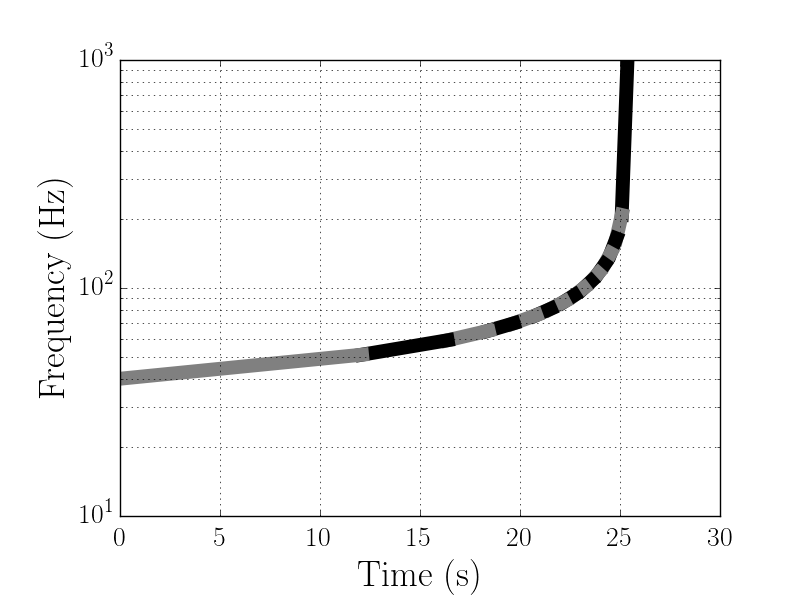
\includegraphics[width=1.0\textwidth]{papers/bns_o1_dev/figures/bin.png}
\caption{\label{fig:chisqbins} 
Approximate boundaries of the 16 bins that make up the time-frequency signal consistency test, as used in S6/VSR2,3, overlaid on the track of a $1.4-1.4M_odot$ BNS waveform. 
}
\end{figure}

\begin{figure}
\centering
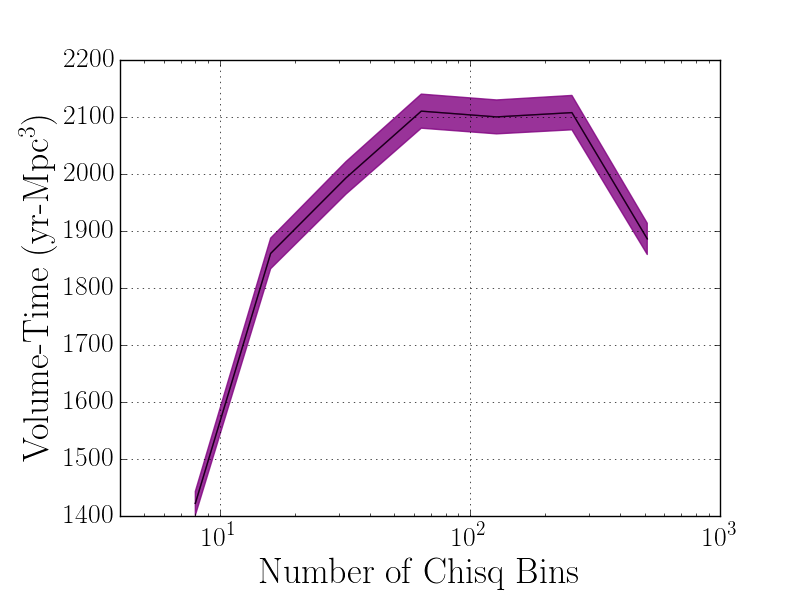
\includegraphics[width=1.0\textwidth]{papers/bns_o1_dev/figures/cb.png}
\caption{\label{fig:vbin} 
The combined VT at inclusive inverse false alarm rate of 1/1000 years as a function of the number of time-frequency bins in the signal-consistency test, for the combined three weeks of analysis, and for an injection population that uniformly covers the parameter space of the non-spinning BNS region, with component masses between $1- 3M_\odot$. There is an $\approx 13\% $ improvement in the analysis sensitivity when using 64-256 bins, as compared to the reference 16 bins.
}
\end{figure}

\begin{figure}
\centering
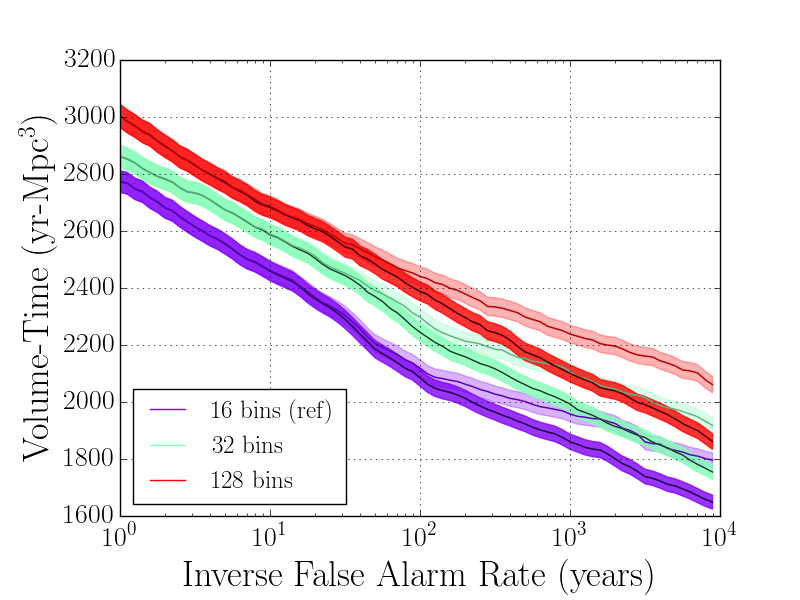
\includegraphics[width=1.0\textwidth]{papers/bns_o1_dev/figures/chisq_combined.png}
\caption{\label{fig:fchisq} 
The combined VT as a function of inverse false alarm rate, for the combined three weeks of analysis, and for an injection population that uniformly covers the parameter space of the non-spinning BNS region, with component masses between $1- 3M_\odot$. Darker colored lines indicate the inclusive IFAR value, while lighter lines show the exclusive IFAR. 
}
\end{figure}

\subsection{Lower-frequency cutoff of the matched filter}

As we have been using data from the sixth LIGO science run, we expect that seismic noise will dominate at low frequencies, and so have used the same 40Hz lower-frequency cutoff used in the S6/VSR2,3 analysis. We can verify that using a 40Hz lower-frequency cutoff does not impact search peformance by constructing

\begin{equation}
V(f_{low}) = \left[ \frac{\int_{f_{low}} \frac{h^{*}(f)h(f)}{S_n(f)} df}{\int_{0} \frac{h^*(f)h(f)}{S_n(f)} df} \right]^3
\end{equation}

where $h(f)$ is a template waveform, $S_n(f)$ is the power spectral densitity, and the quantity $V(f_{low})$ represents the fraction of the optimal volume for a single template
filtered from the lower-frequency cutoff, $f_{low}$. Fig~\ref{fig:flow} shows that filtering from 40Hz only results in only a $1\%$ loss in search volume, for a single 1.4-1.4$M_\odot$ TaylorF2 template, and so it is an appropriate choice for this data.

%The initial ligo noise curves do not caontain significant power below 40Hz for CBC signals, as we progress towards ZDHP, however this will change, and we will need to begin searching with template that begin at a lower frequency. This also implies that they will be longer, and whereas from 40Hz the longest template in our bank which is a 1-1 system was 48s long, it is 95s from 30Hz and 600s from 15 Hz. For O1, we expect that there may be additional power that is worth filtering below 40Hz, however, the increase in correlation length means that there is an increased chance of a filter overlapping a non-gaussian noise event (glitch) that will impact the filter performance. 

%As such, in the case of non-gaussian noise, there is a trade-off between the increased SNR recovery and the increased chance of glitch overlap. If we model this problablity as linearly proportional to the length of the template it can be expressed as, INSERT DEFINITION.


\begin{figure}
\centering
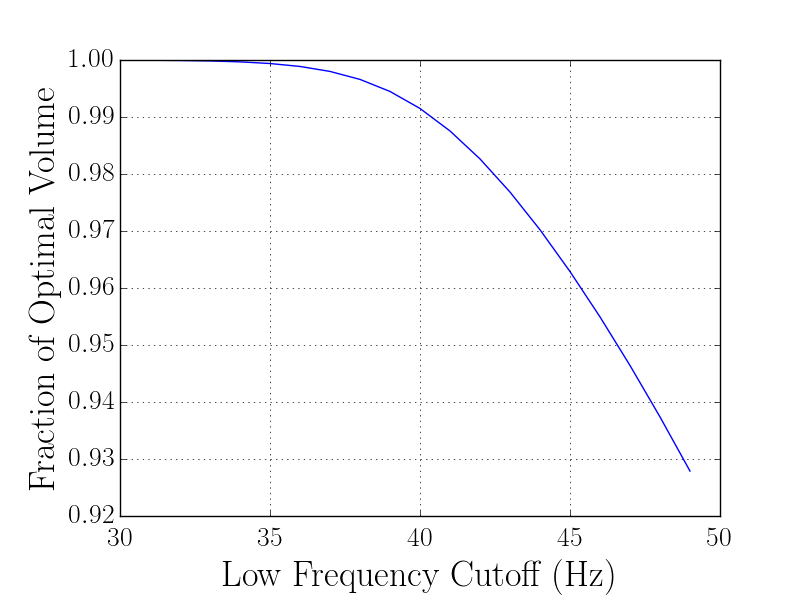
\includegraphics[width=1.0\textwidth]{papers/bns_o1_dev/figures/flow.png}
\caption{\label{fig:flow} 
The fraction of the optimal search volume for a $1.4-1.4 M_\odot$ TaylorF2 BNS waveform, as a function of the lower-frequency cutoff of the matched filter. 
}
\end{figure}

%\subsection{False Alarm Rate vs. Parameter space coverage}
% include for Gaussian noise, S6, and recolored S6 data, % no injection analysis here

\section{Sensitivity to Astrophysical Sources}

In the following sections we compare the sensitivity of tuned BNS analysis we find from sec.~\ref{sec:chisq} to the original filter settings used in Ch.~\ref{ch:single_stage}, and which mimic those used in the S6/VSR2,3 analysis. We consider two choices banks of templates, a \emph{nonspin} template bank designed to be sensitive to mergers where the components have neglible intrinsic angular moment, and an \emph{aligned} template bank which is designed to be sensitive to BNS mergers where the intrinsic angular momentum of the components can be as large as $\chi=0.4$, and is aligned with the binary's orbital angular momentum.

\subsection{Broad distribution of non-spinning sources}

In this section we test the sensitivity of the BNS anysis to broad mass distribution ($1-3 \M_\odot$) of sources where the component neutron stars are non-spinning. The parameter space corresponds to the intended coverage of the non-spinning template bank we have tuned against in \ref{sec:tuning}.  If \ref{fig:nonspin} we show the reference and tuned pipeline configuration using both the aligned spin and nonspin template banks. We see that for either template bank there is a ~25$\%$ increase in search volume using the improved pipeline tunings. Both template banks use the same geometric placement algorithm and required minimal match, and since the injection set is strictly within the boundaries of both template banks, the loss of $\approx 6\%$ loss in search volume when using the aligned spin template bank is due to the increase in background associated with the $\approx 10x$ increase in template bank size.

\begin{figure}
\centering
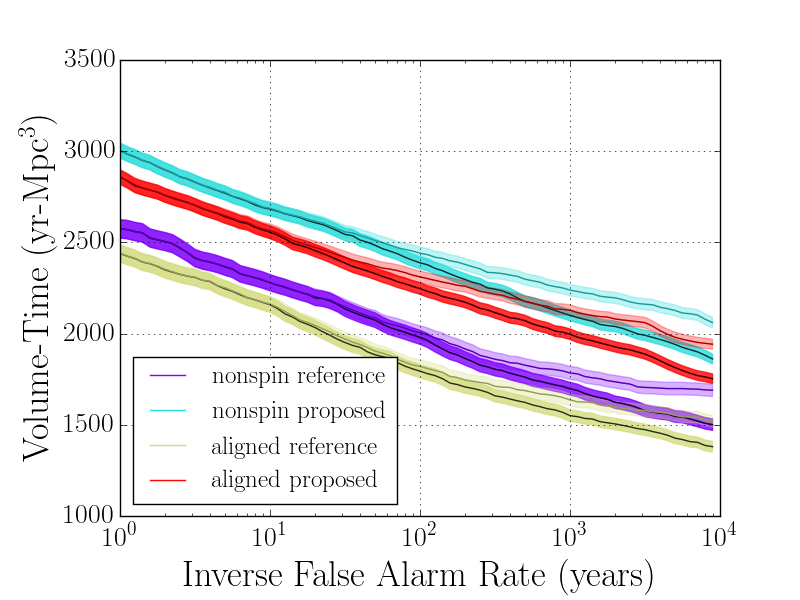
\includegraphics[width=1.0\textwidth]{papers/bns_o1_dev/figures/ns_combined.png}
\caption{\label{fig:nonspin} 
The combined VT as a function of inverse false alarm rate, for the
three sample analysis weeks, for an injection population that uniformly covers parameter space of the non-spinning BNS region, $1- 3M_\odot$. Darker shaded lines indicate the inclusive IFAR value, while lighter lines show the exclusive IFAR. For both the non-spinning template bank and the aligned spin template bank there is $\approx 25 \%$ improvement in search sensitivity.
}
\end{figure}

\subsection{Broad distribution of aligned-spin sources}
\label{sec:baligned}

In this section we choose a distribution of sources drawn unformly from the parameter space that the aligned spin template bank is intended to cover, where each components' mass is between 1 and 3 $\M_\odot$ and the spin magnitude is uniformly distributed between $\chi=$0 and 0.4. The intrinsic spin of each neutron star is restricted to aligned to the orbital angular momentum. One would expected this distribution to be more favourable to the aligned spin template bank than the non-spinning one. We find in \ref{fig:aligned} that the aligned spin template only provides a marginal $\approx 2\%$ improvement in search volume, which we note is close to the measured statistical error. 

\begin{figure}
\centering
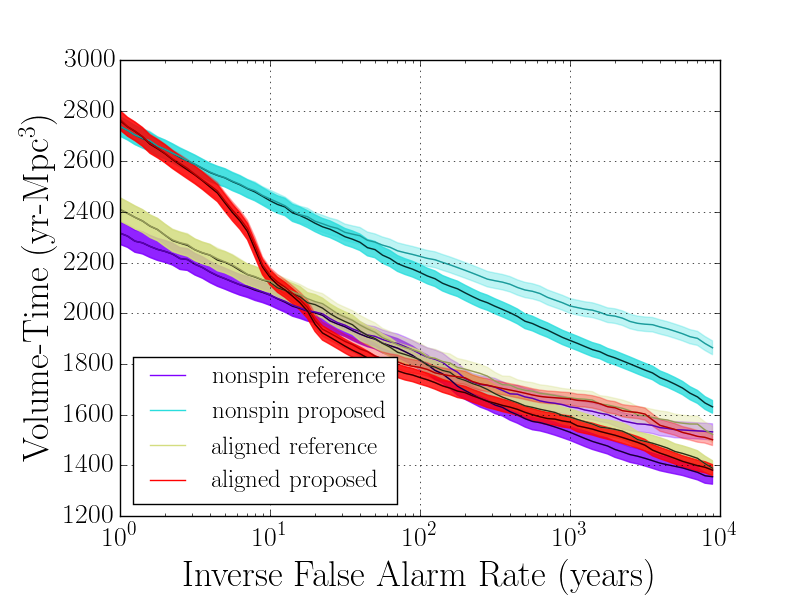
\includegraphics[width=1.0\textwidth]{papers/bns_o1_dev/figures/aligned_combined.png}
\caption{\label{fig:aligned} 
The combined VT as a function of inverse false alarm rate, for the
three sample analysis weeks, for an injection population that uniformly covers parameter space of the aligned spinning BNS region, $1- 3M_\odot$, and $|\chi| <= 0.4$. Darker shaded lines indicate the inclusive IFAR value, while lighter lines show the exclusive IFAR. At a false alarm rate of 1 per 1000 years, the aligned spin template bank improves the overall search sensitivity by only $\approx 2\%$
}
\end{figure}

\subsection{Broad distribution of precessing Sources}

In constrast to the distribution of injections used in sec~\ref{sec:baligned}, we do not expect that coalescing systems will preferentially contain binary neutron stars whose spin is aligned with the orbital angular memoment. In this section, we test the same population of sources, but where the spin angles are isotropically distribued. This will allow the systms to precess, however, as the mass ratio of a BNS systems and the magnitude of the spin is small, the effect of precession is not significant. Although the injection population covers the full range of spin magnitudes, which the algined spin template bank is designed to recover, the nonspinning template bank is marginally more sensitive. Fig.\ref{fig:prec} shows there is an $\approx 1.5\%$ increase in search volume. A source population that is highly weighted towards higly spinning systems would be required for the aligned spin template to substantially improve the search sensitivity over the nonspinning template bank. 

\begin{figure}
\centering
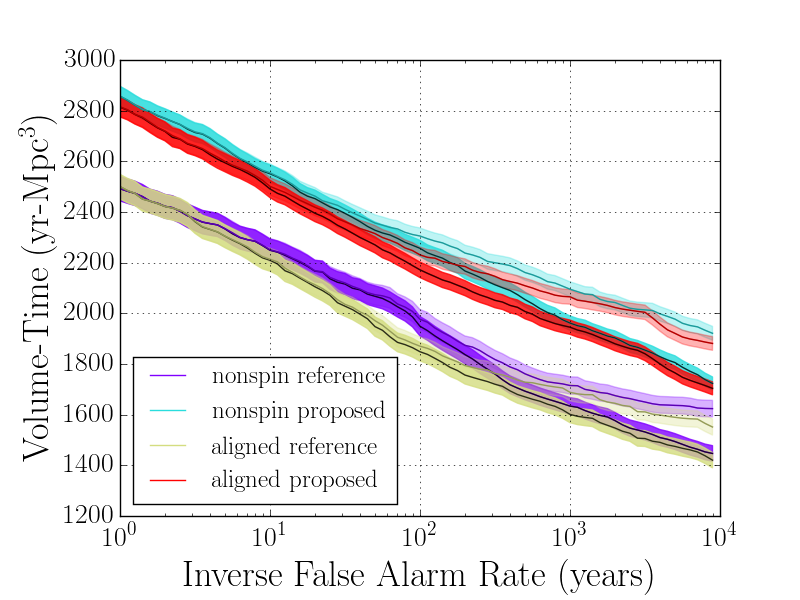
\includegraphics[width=1.0\textwidth]{papers/bns_o1_dev/figures/prec_combined.png}
\caption{\label{fig:prec} 
The combined VT as a function of inverse false alarm rate, for the
three sample analysis weeks, for an injection population that uniformly covers parameter space of the non-spinning BNS region, $1- 3M_\odot$, where
the spin angles are isotropically distributed, and the spin magnitude $|\chi| < 0.4$. Darker shaded lines indicate the inclusive IFAR value, while lighter lines show the exclusive IFAR. There is a negligible difference in search performance between using the aligned spin and nonspinning template bank.
}
\end{figure}

\subsection{Astrophysically-motivated Conservative Source Distribution}

We test the focused BNS anaysis against an estimate of astrophysical sources using an injection population drawn from a conservative range of mass and spin distributions. Based on the population of observed BNS sources, as noted in sec.~\ref{atro:bns}, we draw injections from a populution with a Gaussian distribution of component masses centered on $1.40 \M_\odot$, and a standard deviation of 0.13. The intrinsic spin of each neutron star is chosen from a uniform distribution of spin magnitudes $|\chi| < 0.05$, and an isotropic distribution of spin angles. 

We clearly see in fig~\ref{fig:rest} that a search using only a non-spinning template bank yields a $\approx{7\%}$ improvment in search sensitvity over one that covers an expansive spin range. If the true distribution of signals matches the expectations from current observations, then a non-spinning template bank is the preferred option. Note, that future work should investigate alternate possibilities for incorporating expected population distributions into the search directly, wich may allow a more fine-grained inclusion of spinning regions of the parameter space, while sacrificing less in overall sensitivity to the most likely signals.

\begin{figure}
\centering
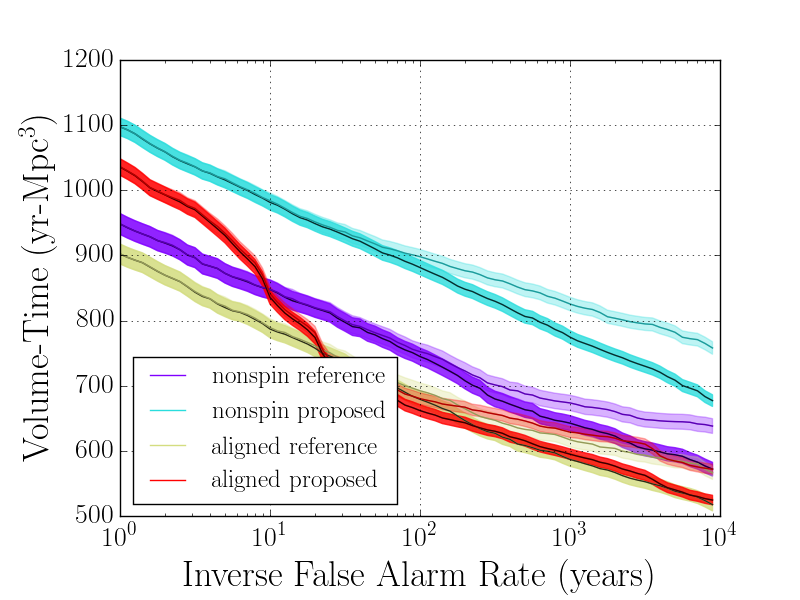
\includegraphics[width=1.0\textwidth]{papers/bns_o1_dev/figures/rest_combined.png}
\caption{\label{fig:rest} 
The VT as a function of inverse false alarm rate, for the
three sample analysis weeks, for an astrophysically-motivated conservative mass and spin distribution. Darker shaded lines indicate the inclusive IFAR value, while lighter lines show the exclusive IFAR. There is an $\approx 7\%$ drop in sensitivity when using the full aligned spin template bank when compared to the the non-spinning
template bank.}
\end{figure}

\section{Conclusions}

We have presented a new pipeline specifically targeted for the detection of gravitational-waves from binary neutron star sources in LIGO data. Using the single stage search pipeline we investigated the configuration choices used for PSD estimation, SNR thresholds, low frequency cutoff, and $\chi^2$ bins used within the ranking statistic. To assess the sensitivity, we develop a method to measure the false alarm rate of possible signals, and introduce the concept of both the inclusive and exclusive FAR measures. We find that for S6 data, the choices for low frequency cutoff at 40Hz, and the SNR threshold at 5.5, as used in prior S6/VSR2,3 searches for BNS sources, were appropriate. Additionally, we find that for a two detector search conducted using the Hanford and Livingston observatories, decreasing the SNR threshold below 5.3 will not result in any gain in search sensitivity using the conservative inclusive IFAR. In sec~\ref{sec:psd} and sec~\ref{sec:chisq} we show significant improvements in search sensitivity for BNS sources by retuning the number of PSD samples per estimate, and the number of bins used in the signal consistance test, respectively. We find a total $25\%$ increase in the detection rate of BNS systems when using the retuned BNS search over a BNS search that uses the configuration used in S6/VSR2,3. We also find that using an aligned spin template bank marginally decreases the sensitivity 
to BNS mergers for conservative estimates of the BNS populations when comparing to a bank of stictly non-spinning templates. As these tuning significantly differ from those used in the wider lowmass search performed in S6/VSR2,3, we propose that a focused, non-spinning search for binary neutron stars be conducted for aLIGO and AdV.

\label{sec:conclusions}
